\documentclass[parskip=full]{scrartcl}
\usepackage[T1]{fontenc}    % avoid garbled Unicode text in pdf
\usepackage[utf8]{inputenc} % use utf8 file encoding for TeX sources
\usepackage[german]{babel}  % german hyphenation, quotes, etc
\usepackage{hyperref}       % detailed hyperlink/pdf configuration
\hypersetup{                % ‘texdoc hyperref‘ for options
pdftitle={PSE: Entwicklung eines relationalen Debuggers - Pflichtenheft},%
,%
}
\usepackage{graphicx}       % provides commands for including figures
\usepackage{csquotes}       % provides \enquote{} macro for "quotes"
\usepackage[nonumberlist]{glossaries}     % provides glossary commands
\usepackage{enumitem}
\usepackage{xcolor}
\newcommand\frage[1]{\textcolor{red}{#1}}


\font\myfont=cmr12 at 20pt

\title{
	\vspace{2cm}
	\myfont 
	Praxis der Softwareentwicklung:\\ 
	Entwicklung eines relationalen Debuggers\\
}
\subtitle{
	\vspace{1cm}
	\myfont
	Entwurfsdokument
}
\author{
	\vspace{1cm} \\
	Benedikt Wagner\\
	\texttt{udpto@student.kit.edu}
	\and \vspace{1cm} \\ Chiara Staudenmaier\\
	\texttt{uzhtd@student.kit.edu}
	\and Etienne Brunner\\
	\texttt{urmlp@student.kit.edu}
	\and Joana Plewnia\\
	\texttt{uhfpm@student.kit.edu} 
	\and Pascal Zwick\\
	\texttt{uyqpk@student.kit.edu}
	\and Ulla Scheler\\
	\texttt{ujuhe@student.kit.edu}
	\vspace{1cm}
	\and Betreuer: Mihai Herda, Michael Kirsten
	\vspace{4cm}
}


\begin{document}
\clearpage
\maketitle
\pagenumbering{gobble}
\newpage

\tableofcontents
\newpage
\pagenumbering{arabic}
%Eventuell Fußnoten generieren
\section{Einleitung}
%Einleitung mit grobem Überblick. Dieser Abschnitt soll an das Pflichtenheft anschließen.
Dieses Dokument dokumentiert die Ergebnisse der Entwurfsphase (\textit{28.11.-22.12.2017}) im Rahmen
des Moduls Praxis der Softwareentwicklung (PSE) am Lehrstuhl \enquote{Anwendungsorientierte formale Verifikation - Prof. Dr. Beckert} am Karlsruher Institut für Technologie (KIT).\\
Hierbei handelt es sich um den Entwurf des Produkts \textit{DIbugger}, welches im Pflichtenheft definiert wurde. 
Das Entwurfsdokument beschreibt die Paketeinteilung, Beschreibung der Klassen und Abläufe und genaue Spezifikation der Abhängigkeiten und Kernkomponenten. 
\\Die Implementierung während der Implementierungsphase (\textit{09.01.-02.02.2018}) wird anhand der Vorgaben in diesem Dokument durchgeführt. \\
Hierbei werden das Geheimnisprinzip und Lose Kopplung berücksichtigt, um für erhöhte Verständlichkeit
zu sorgen. %TODO wir sollten noch erklären, wie und wo genau wir diese Prinzipien sicherstellen

\vspace{1cm}
\begin{figure}[!h]
\centering

\includegraphics[width=0.8\textwidth]{../Plichtenheft/logo_nongi.png}
\caption{Produktlogo}
\end{figure}

\newpage


\section{Paketeinteilung} %eventuell fällt jemandem ein besserer Titel ein
%Paketdiagramm, Erläuterung der Einteilungsentscheidung, Schnittstellen

\subsection{Übersicht}

\begin{figure}[!h]
\centering
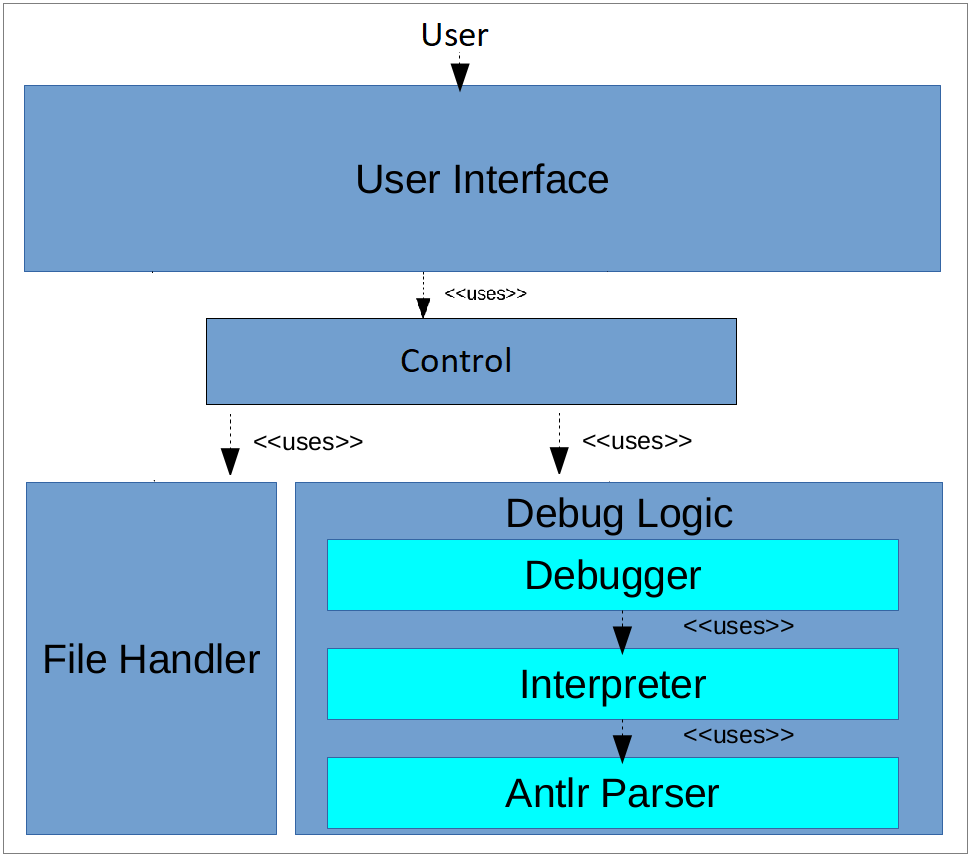
\includegraphics[scale=0.35]{../Plichtenheft/Architektur.png} \\
\caption{Architekturdiagramm}
\end{figure}
Das Produkt ist aufgeteilt in die Pakete \textit{Control}, \textit{UserInterface}, \textit{FileHandler} und \textit{DebugLogic}.
Die \textit{DebugLogic} besteht aus den Unterpaketen \textit{Debugger}, \textit{Interpreter} und
\textit{AntlrParser}.\\
Hierbei wird das Architekturmuster Model-View-Controller (MVC) eingesetzt, um einen flexiblen Programmentwurf zu ermöglichen und die Erweiterbarkeit des Produkts sicher zu stellen. Die Pakete \textit{DebugLogic} und \textit{FileHandler} sind hierbei das Modell, welches die darzustellenden Daten enthält. Das \textit{UserInterface} ist die Präsentationsschicht, welche Benutzereingaben annimmt und die darzustellenden Werte über ein Beobachtermuster erhält. Die Steuerung, welche Benutzereingaben von der Präsentationsschicht erhält und diese auswertet, wird vom \textit{Control}-Paket bereitgestellt. \\
Alle Pakete stellen ihre Funktionalität über Fassadenklassen nach aussen zur Verfügung. Die genauen Schnittstellen sind also durch diese Klassen definiert.

\newpage

\subsection{User Interface}
\paragraph{Aufgaben} Das Paket \textit{UserInterface} stellt die Möglichkeit zur Kommunikation des Nutzers mit dem Produkt dar. Hierbei dient dieses Paket als View Teil des MVC-Konzepts.
\paragraph{Schnittstellen} 
\begin{itemize}
\item Angebotene Schnittstellen:\\
Es wird eine Fassade angeboten, welche es ermöglicht, Variablen, Programmtexte und Eingaben anzuzeigen.
\item Genutzte Schnittstellen:\\
Dieses Paket nutzt die Fassade des Paketes \textit{Control} und deren angebotenen Schnittstellen.
\end{itemize}
\paragraph{Benutztrelation} Das Paket \textit{UserInterface} benutzt die Control-Fassade, um an jegliche, durch den Benutzer angeforderte, Information zu gelangen, bzw. das vom Benutzer geforderte auszuführen. %ich versteh den Satz nicht..


\subsection{Control}
\paragraph{Aufgaben}
    Das Paket \textit{Control} entspricht dem Kontrollsubsystem gemäß dem Architekturstil MVC.\\
    Es dient der Entgegennahme von Benutzerinteraktionen auf der Benutzeroberfläche und Steuerung der Interaktion zwischen den
    Subsystemen \textit{UserInterface} und \textit{DebugLogic}.\\
    Schaltflächen, sowie Eingabefelder sind Teil des Kontrollsubsystems und werden im Paket 
    \textit{UserInterface} mit Präsentationskomponenten wie dem Variableninspektor zusammengefasst.\\
\paragraph{Schnittstellen}
    Die vom Paket bereitgestellten Methoden sind über eine Fassade aufrufbar.\\
    Die Methoden verursachen Zustandsveränderung des Datenmodells \textit{DebugLogic}.\\
    Beispielsweise kann das Modell aufgefordert werden, einen eingegebenen Quelltext oder spezifizierten Haltepunkt
    zu speichern oder zu löschen.\\
    Weiter kann das Modell dazu aufgefordert werden, datenbezogene Aktionen auszuführen wie
    das Starten eines Debugvorgangs, oder Durchführen eines Einzelschrittes. Zusätzlich steuert das Paket Speicher- oder Ladeaufträge an das Paket \textit{FileHandler} geben. 
    %TODO Diesen komischen Satz noch zu einem sinnvollen, deutschen machen.
\paragraph{Benutztrelation}
    \textit{Control} benutzt die Pakete \textit{DebugLogic} und \textit{FileHandler}.%Warum?

\subsection{File Handler}
\paragraph{Aufgaben}
Das Paket FileHandler stellt die Funktionalität zum Lesen, Schreiben, Parsen und Interpretieren von sämtlichen Dateien bereit und siedelt sich im Model Teil des MVC-Konzepts an.
Dabei wandelt dieser eine Konfigurationsdatei, welche auf dem Dateisystem gespeichert ist, in eine virtuelle Datei um.
Diese besteht aus einer Klassenstruktur, welche äquivalent zur Definition des Speicherformats ist, also Zuweisungen und Blöcke.
Weiter erzeugt der FileHandler Objekte der Konfigurations-, Sprach- und Einstellungsdateien und kann diese nach außen weitergeben.
\paragraph{Schnittstellen}
\begin{itemize}
\item Genutzte Schnittstellen: \\
Der FileHandler benötigt keine Schnittstellen anderer Programmpakete, da er an unterster Stelle in der Benutztrelation steht.
\item Angebotene Schnittstellen: \\
Es werden eine Fassade und drei Klassen angeboten.
Diese repräsentieren die Dateien für Produkteinstellungen, Sprachen (Übersetzungen der GUI) und Laufkonfigurationen.

\end{itemize}
\paragraph{Benutztrelation}
Der FileHandler hat keine Unterpakete
%TODO echt keine Zwick?  und steht an unterster Stelle der Benutztrelation.
Somit entstehen auch keine Abhängigkeiten zu anderen Paketen.

\subsection{Debug Logic}
Das Paket \textit{DebugLogic} stellt den Model Teil der MVC Architektur dar. Die interne Struktur des Paketes ist eine intransparente 3-Schichten-Architektur.\\
Die unterste Schicht stellt das Subpaket \textit{DebugLogic.AntlrParser} dar. Es erzeugt aus einfachen Zeichenketten Ableitungsbäume nach den Ableitungsregeln der in \ref{FormSpez} gegebenen Grammatiken.\\ Darauf aufbauend in der mittleren Schicht finden sich die Subpakete \textit{DebugLogic.TraceGenerator} und \textit{DebugLogic.RelationalExpressionGenerator}, die beide die Aufgabe haben, diese Ableitungsbäume durch interpretieren in eine abstrakte und leicht handhabbare Form zu bringen. Da beide Subpakete eine gemeinsame Schicht darstellen, findet hier auch ein hohes Maß an Kommunikation statt. \\ In der obersten Schicht ist das Subpaket \textit{DebugLogic.Debugger} angesiedelt. Dieses nutzt die abstrakten Repräsentationen und führt den eigentlichen Debugprozess darauf aus.
\subsubsection{Debugger}
\subparagraph{Aufgaben}
Der Debugger nutzt die von den Subpaketen \textit{DebugLogic.TraceGenerator} und \textit{DebugLogic.RelationalExpressionGenerator} erzeugten Informationen, um Watch-Expressions und bedingte Breakpoints auszuwerten, sowie die üblichen Debugmechanismen zu steuern.
\subparagraph{Schnittstellen}
Als oberste Schicht des Paketes \textit{DebugLogic} stellt dieses Subpaket die gleichen Schnittstellen wie die DebugLogic bereit. Diese können in \ref{Klassen} der entsprechenden Fassadenklasse entnommen werden.
\subparagraph{Benutztrelation} 
%Das Subpaket benutzt die Subpakete \textit{DebugLogic.TraceGenerator} und \textit{DebugLogic.RelationalExpressionGenerator}.
%Um die üblichen Debugmechanismen wie Schritte und Weiter durchführen zu können, nutzt dieses Subpaket den vom Subpaket \textit{DebugLogic.TraceGenerator} bereitgestellten Iterator. 
%Um WatchExpressions und bedingte Breakpoints auszuwerten und zu repräsentieren, nutzt dieses Subpaket die vom Subpaket \textit{DebugLogic.RelationalExpressionGenerator} bereitgestellte abstrakte Repräsentationen.


Um die üblichen Debugmechanismen wie Schritte und Weiter durchführen zu können, nutzt dieses Subpaket den vom Subpaket \textit{DebugLogic.Interpreter} bereitgestellten Trace-Iterator. 
Um WatchExpressions und bedingte Breakpoints auszuwerten und zu repräsentieren, nutzt dieses Subpaket die vom Subpaket \textit{DebugLogic.Interpreter} bereitgestellte abstrakte Repräsentationen.

\subparagraph{Interpreter}
Dieses Paket ist dafür verantwortlich, die bereits vom \textit{DebugLogic.AntlrParser}  geparsten Nutzereingaben so zu verarbeiten, dass der \textit{DebugLogic.Debugger} damit weiterarbeiten kann. Nimmt das Paket vom \textit{DebugLogic.AntlrParser} den Quelltext eines (WLang-) Programms entgegen, erzeugt es einen Pfad über den gesamten Programmfluss des Programms, sodass später darüber iteriert werden kann. Nimmt das Paket Zeichenketten entgegen, die Watch-Expressions und bedingte Breakpoints beschreiben, interpretiert es diese und stellt sie abstrakt dar.
Innerhalb dieses Paketes wird auch auf semantische Fehler geprüft, etwa das Fehlen eines return-Statements.

%TODO ist Zeichenketten hier schon präzise genug? Wie sehen die Zeichenketten aus, wenn sie aus Antlr herauskommen? Weiter oben heißt es nämlich, dass alles vom User erst in Antlr geparst wird.

\subparagraph{Schnittstellen}
\begin{itemize}
\item Angebotene Funktionalität:\\
Stellt einen Iterator über den Ausführungspfad eines gegebenen Programmes zur Verfügung. Erzeugt aus gegebenen Zeichenketten für Watch-Expressions und bedingte Breakpoints eine abstrakte Repräsentation, sodass diese dann leicht ausgewertet werden kann.

\item Genutzte Funktionalität:\\
Nutzt Syntax-Prüfung und Syntaxbaum-Erzeugung des Subpakets \textit{DebugLogic.AntlrParser}. 
\end{itemize}

\subparagraph{Benutztrelation} 
Dieses Unterpaket benutzt das Unterpaket \textit{DebugLogic.AntlrParser}, um damit aus den reinen Zeichenketten einen Syntaxbaum gemäß der in \ref{FormSpez} gegebenen Grammatik für die Sprache WLang erzeugen zu lassen.

%\subsubsection{TraceGenerator}
%\subparagraph{Aufgaben}
%Dieses Subpaket nimmt den Quelltext eines WLang-Programms entgegen und hat die Aufgabe, einen Pfad über den gesamten Programmfluss dessen zu erzeugen, sodass später darüber iteriert werden kann. Dazu gehört auch das Prüfen auf semantische Fehler, etwa das Fehlen eines return-Statements. \\
%\subparagraph{Schnittstellen}
%\begin{itemize}
%\item Angebotene Funktionalität:\\
%Stellt einen Iterator über den Ausführungspfad eines gegebenen Programmes zur Verfügung.
%\item Genutzte Funktionalität:\\
%Nutzt Syntax-Prüfung und Syntaxbaum-Erzeugung des Subpakets \textit{DebugLogic.AntlrParser}. 
%\end{itemize}
%
%%TODO Schnittstellen in Form von Facade
%\subparagraph{Benutztrelation} 
%Das Unterpaket benutzt das Unterpaket \textit{DebugLogic.AntlrParser}, um damit aus den reinen Zeichenketten einen Syntaxbaum gemäß der in \ref{FormSpez} gegebenen Grammatik für die Sprache WLang erzeugen zu lassen. Auf dieser Vorraussetzung baut die Arbeit des Subpakets auf.
%\subsubsection{Relational Expression Generator}
%\subparagraph{Aufgaben}
%Dieses Subpaket nimmt Zeichenketten, die Watch-Expressions und bedingte Breakpoints beschreiben, entgegen und hat die Aufgabe, diese zu interpretieren. Dazu wird in diesem Paket eine abstrakte Darstellung dieser erzeugt.
%\subparagraph{Schnittstellen}
%\begin{itemize}
%\item Angebotene Funktionalität:\\
%Erzeugt aus gegebenen Zeichenketten für Watch-Expressions und bedingte Breakpoints eine abstrakte Repräsentation, sodass diese dann leicht ausgewertet werden kann.
%\item Genutzte Funktionalität:\\
%Nutzt Syntax-Prüfung und Syntaxbaum-Erzeugung des Subpakets \textit{DebugLogic.AntlrParser}. 
%\end{itemize}
%%TODO Schnittstellen in Form von Facade
%\subparagraph{Benutztrelation} 
%Das Unterpaket benutzt das Unterpaket \textit{DebugLogic.AntlrParser}, um damit aus den reinen Zeichenketten einen Syntaxbaum gemäß der in \ref{FormSpez} gegebenen Grammatik für Watch-Expressions und Bedingte Breakpoints erzeugen zu lassen. Auf dieser Vorraussetzung baut die Arbeit des Subpakets auf.
\subsubsection{Antlr Parser}
Dieses Paket beinhaltet nur Klassen, welche von der Antlr Bibliothek auf Basis der WLang Grammatik generiert werden und somit nicht per Hand geschrieben sind.
\subparagraph{Aufgaben}
Dieses Unterpaket parst die Eingaben des Nutzers (d.h. sowohl Programmtexte als auch Variablen und Ausdrücke für bedingte Breakpoints und Watch-Expressions) gemäß der in \ref{FormSpez} gegebenen Grammatik.

\subparagraph{Schnittstellen}
\begin{itemize}
\item Angebotene Funktionalität:\\
Prüft die textbasierten Eingaben des Nutzers auf Übereinstimmung mit der gegebenen Grammatik und erzeugt aus der Eingabe einen ablaufbaren Syntaxbaum, der dann vom Unterpaket \textit{DebugLogic.RelationalExpressionGenerator} weiter ausgewertet werden kann.
\item Genutzte Funktionalität:\\
Benötigt keine Schnittstellen anderer Programmpakete, da das Paket an unterster Stelle der Benutztrelation steht.
\end{itemize}
\subparagraph{Benutztrelation}
Der Antlr Parser hat keine Unterpakete und steht an unterster Stelle der Benutztrelation. Somit entstehen keine Abhängigkeiten zu anderen Paketen.

\section{Beschreibung wichtiger Klassen}\label{Klassen}
Detaillierte Beschreibung aller Klassen. Das beinhaltet (JavaDoc) Beschreibungen zu allen Me-
thoden, Konstruktoren, Packages und Klassen. Was hier nicht reingehört sind private Felder
und Methoden. Das sind Implementierungsdetails.

\subsection{Klassen im Paket \enquote{User Interface}}
\paragraph{Fassade}
\begin{itemize}
\item[Klassenbeschreibung] Die Fassade der Benutzeroberfläche (GUIFacade) dient zur Kommunikation mit den anderen Paketen. Um die Benutzeroberfläche einfach austauschen zu können, ist nur die Fassade mit den anderen Paketen verbunden, sodass alle anderen Klassen im Paket User Interface einfach ausgetauscht werden können.
\item[Methoden]
\begin{itemize}
\item showProgramText(String programText, int id): ermöglicht es einen Programmtext in einem bestimmten Programmfeld (durch ID gekennzeichnet) anzuzeigen.
\item
\end{itemize}
\end{itemize}

\subsection{Klassen im Paket \enquote{Control}}

\subsubsection{Unterpaket Debugger}

\subsubsection{Unterpaket Interpreter}

\subsubsection{Unterpaket AntlrParser}

\subsection{Klassen im Paket \enquote{DebugLogic}}

\subsection{Klassen im Paket \enquote{FileHandler}}

\subsubsection{Unterpaket FileHandler.Facade}
\paragraph{FileHandlerFacade}
\begin{itemize}
\item Klassenbeschreibung: \\
Speichert alle verfügbaren Sprachen und hilft bei der Erzeugung von Konfigurationsdateien.
\item loadConfig(File file) : ConfigurationFile \\
Lädt die angegebene Datei als Konfigurationsdatei und gibt diese zurück.
\item saveConfig(ConfigurationFile config) \\
Speichert die angegebene Konfiguration an den darin gespeicherten Dateipfad.
\item getPropertiesFile() : PropertiesFile \\
Gibt die im Voraus geladene Einstellungsdatei zurück.
\item getLanguages() : List<String> \\
Gibt alle Sprachnamen in einer Liste als String zurück.
\item getLanguageFile(String langID) : LanguageFile \\
Gibt die zur langID passende Sprachdatei zurück, falls diese existiert,
sonst wird eine LanguageNotFoundException geworfen.
\end{itemize}

\paragraph{ConfigurationFile}
\begin{itemize}
\item Klassenbeschreibung: \\
Diese Klasse speichert eine Konfiguration des Debuggers.
\item getSystemFile() : File \\
Gibt ein java.io.File Objekt zurück, welchen die Datei im Dateisystem des Nutzers repräsentiert.
\item getProgramText(int programID) : String \\
Gibt den Programmtext von Programm programID als String zurück.
\item getStepSize(int programID) : int \\
Gibt die Schrittgröße von Program programID zurück.
\item getInputValue(int programID, String identifier) : String \\
Gibt den Eingabewert von Programm programID für die Variable identifier zurück, falls diese existeirt,
sonst wird null zurückgegeben.
\item getLatestExecutionLine(int programID) : int \\
Gibt die Position von Programm programID im Programmablaufbaum als int zurück. %TODO bessere erklärung
\item getVariablesOfInspector(int programID) : List<String> \\
Gibt eine Liste von variablen Namen zurück, welche im Variablen Inspektor eingeblendet sind.
\item getWEScopeBegin(int expressionID) : List<int> \\
Gibt eine Liste der Anfanggrenze der Bereichsintervalle für die WatchExpression expressionID zurück
\item getWEScopeEnd(int expressionID) : List<int> \\
Gibt eine Liste der Endgrenze der Bereichsintervalle für die WatchExpression expressionID zurück.
\item getCBScopeBegin(int breakpointID) : List<int> \\
Äquivalente Funktion für bedingte Breakpoints zu getWEScopeBegin
\item getCBScopeEnd(int breakpointID) : List<int> \\
Äquivalente Funktion für bedingte Breakpoints zu getWEScopeEnd
\item getBreakpoints(int programID) : List<int> \\
Gibt eine Liste der Zeilen der Breakpoints für Programm programID zurück.
\end{itemize}

\paragraph{PropertiesFile}
\begin{itemize}
\item Klassenbeschreibung: \\
Diese Klasse speichert die Einstellungen des Debuggers.
\item getSelectedLanguage() : String \\
Gibt den SprachIdentifier der eingestellten Sprache zurück.
\item getLastConfigurationFile() : ConfigurationFile \\
Gibt eine Repräsentation der zuletzt aktiven Konfiguration zurück.
\item getMaxWhileIterations() : int \\
Gibt die eingestellte Obergrenze für Schleifendurchläufe wieder.
\item getMaxFunctionCalls() : int \\
Gibt die eingestelle Obergrenze für Funktionsaufrufe wieder.
\end{itemize}

\paragraph{LanguageFile}
\begin{itemize}
\item Klassenbeschreibung: \\
Stellt eine Übersetzung der GUI zu einer bestimmtem Sprache bereit.
\item getTranslation(String textID) : String \\
Gibt den Text (Übersetzung) zu der übergebenen textID zurück.
\end{itemize}

\paragraph{FileReader}%TODO
\begin{itemize}
\item Klassenbeschreibung: \\
Dient als Schnittstelle von der FileHandlerFacade zum Dateisystem für das Lesen von verschiedene Dateiformate.
\end{itemize}

\paragraph{FileWriter}%TODO
\begin{itemize}
\item Klassenbeschreibung: \\
Dient als Schnittstelle von der FileHandlerFacade zum Dateisystem für das Schreiben in verschiedene Dateiformate.
\end{itemize}

\subsubsection{Unterpaket FileHandler.RDBF}

\subsection{Klassen im Paket \enquote{Exceptions}} 
...
\section{Verwendete Design Patterns}

\subsection{Patterns im Paket User Interface}
Durch die Nutzung von Swing besteht der Grundaufbau des User Interfaces aus einem Kompositum. 
Durch anonyme Instanzen von Action Listenern wird das Befehlsmuster implementiert. \\
Des Weiteren werden die Entwurfsmuster Vererbung (z.B. DebuggerPopUp und ErrorPopUp) und Beobachter (durch das MVC-Konzept vorgegeben) in den Klassen ExpressionPanel und ProgramPanel implementiert.
Die Klassen CondBreakpointPanel und WatchExpressionPanel stellen Singletons dar.
\subsection{Patterns im Paket Control}
\subsection{Patterns im Paket Debug Logic}
\subsection{Patterns im Paket File Handler}

\newpage
\section{Charakteristische Abläufe}
In diesem Kapitel werden charakteristische Abläufe des Produkts, wie der erste Programmaufruf und die
Anwendungsfälle, anhand von Sequenzdiagrammen dargestellt und erklärt.
 %TODO Auf Klassen oder Pakete in Beschreibung aller Klassen verweisen

\subsection{Erster Programmaufruf}
\begin{figure}[!h]
\centering
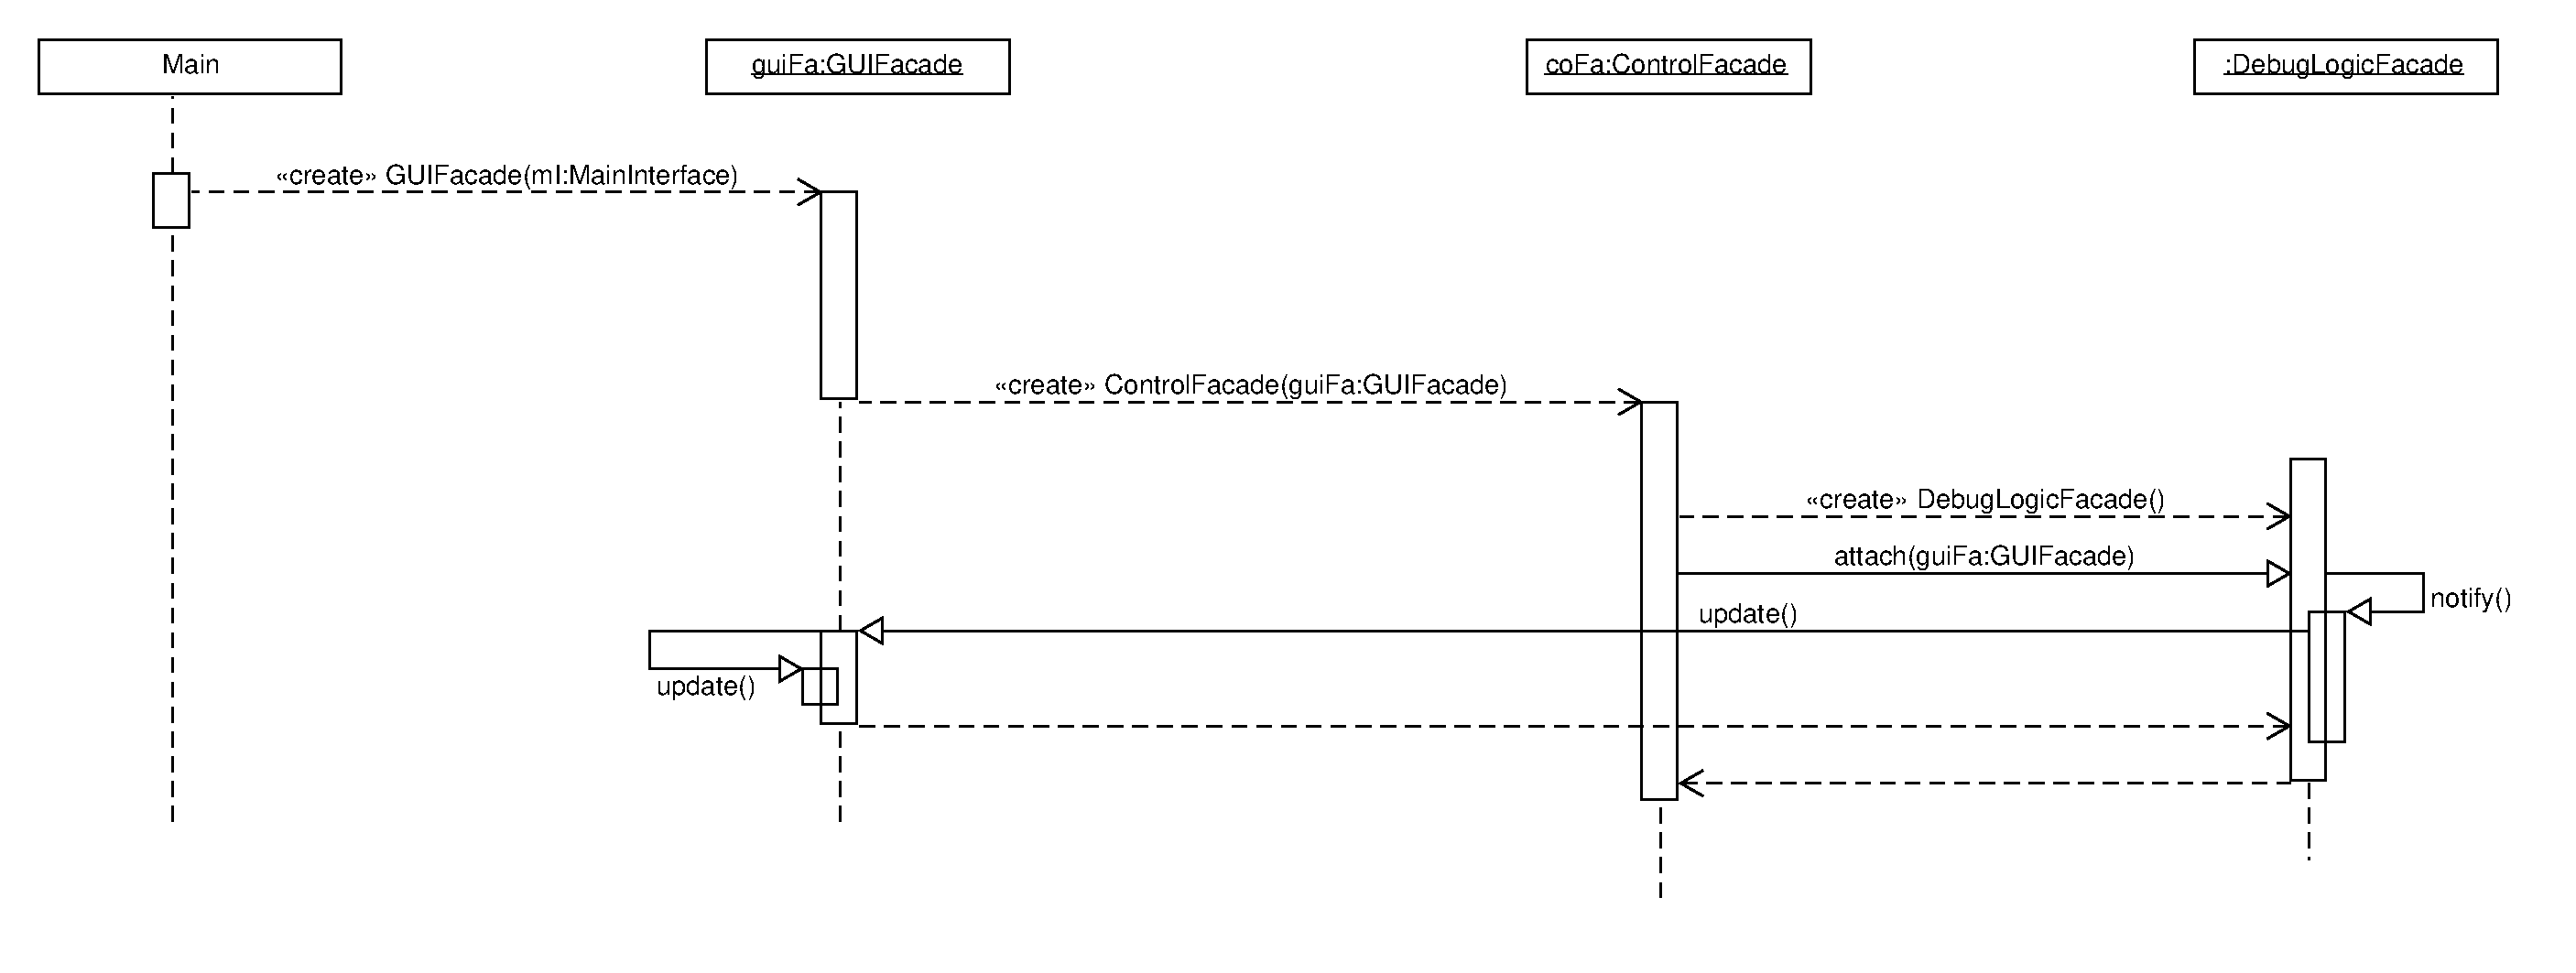
\includegraphics[width=0.8\textwidth]{diagrammIdeenUmlet/SequenceDiagrams/seq_firstCallPDF.pdf}
\caption{Sequenzdiagramm: Erster Programmaufruf}
\end{figure}
Wird das Produkt gestartet, erstellt die Main-Methode des MainInterface die GUIFacade und übergibt sich selbt.
Die GUIFacade speichert das MainInterface und erstellt ihrerseits die ControlFacade, welche wiederum
die DebugLogicFacade erstellt.
Die ControlFacade und DebugLogicFacade erstellen intern Instanzen der Klassen ihrer Pakete. \\
Die GUIFacade wird bei diesem Prozess bis zur DebugLogic weitergereicht, um dort als Observer angemeldet werden
zu können. Wird später dann zum Beispiel ein Breakpoint hinzugefügt, wird die GUIFacade benachrichtigt und
kann sich updaten.

\newpage
\subsection{Konfigurationsdatei laden}
\begin{figure}[!h]
\centering
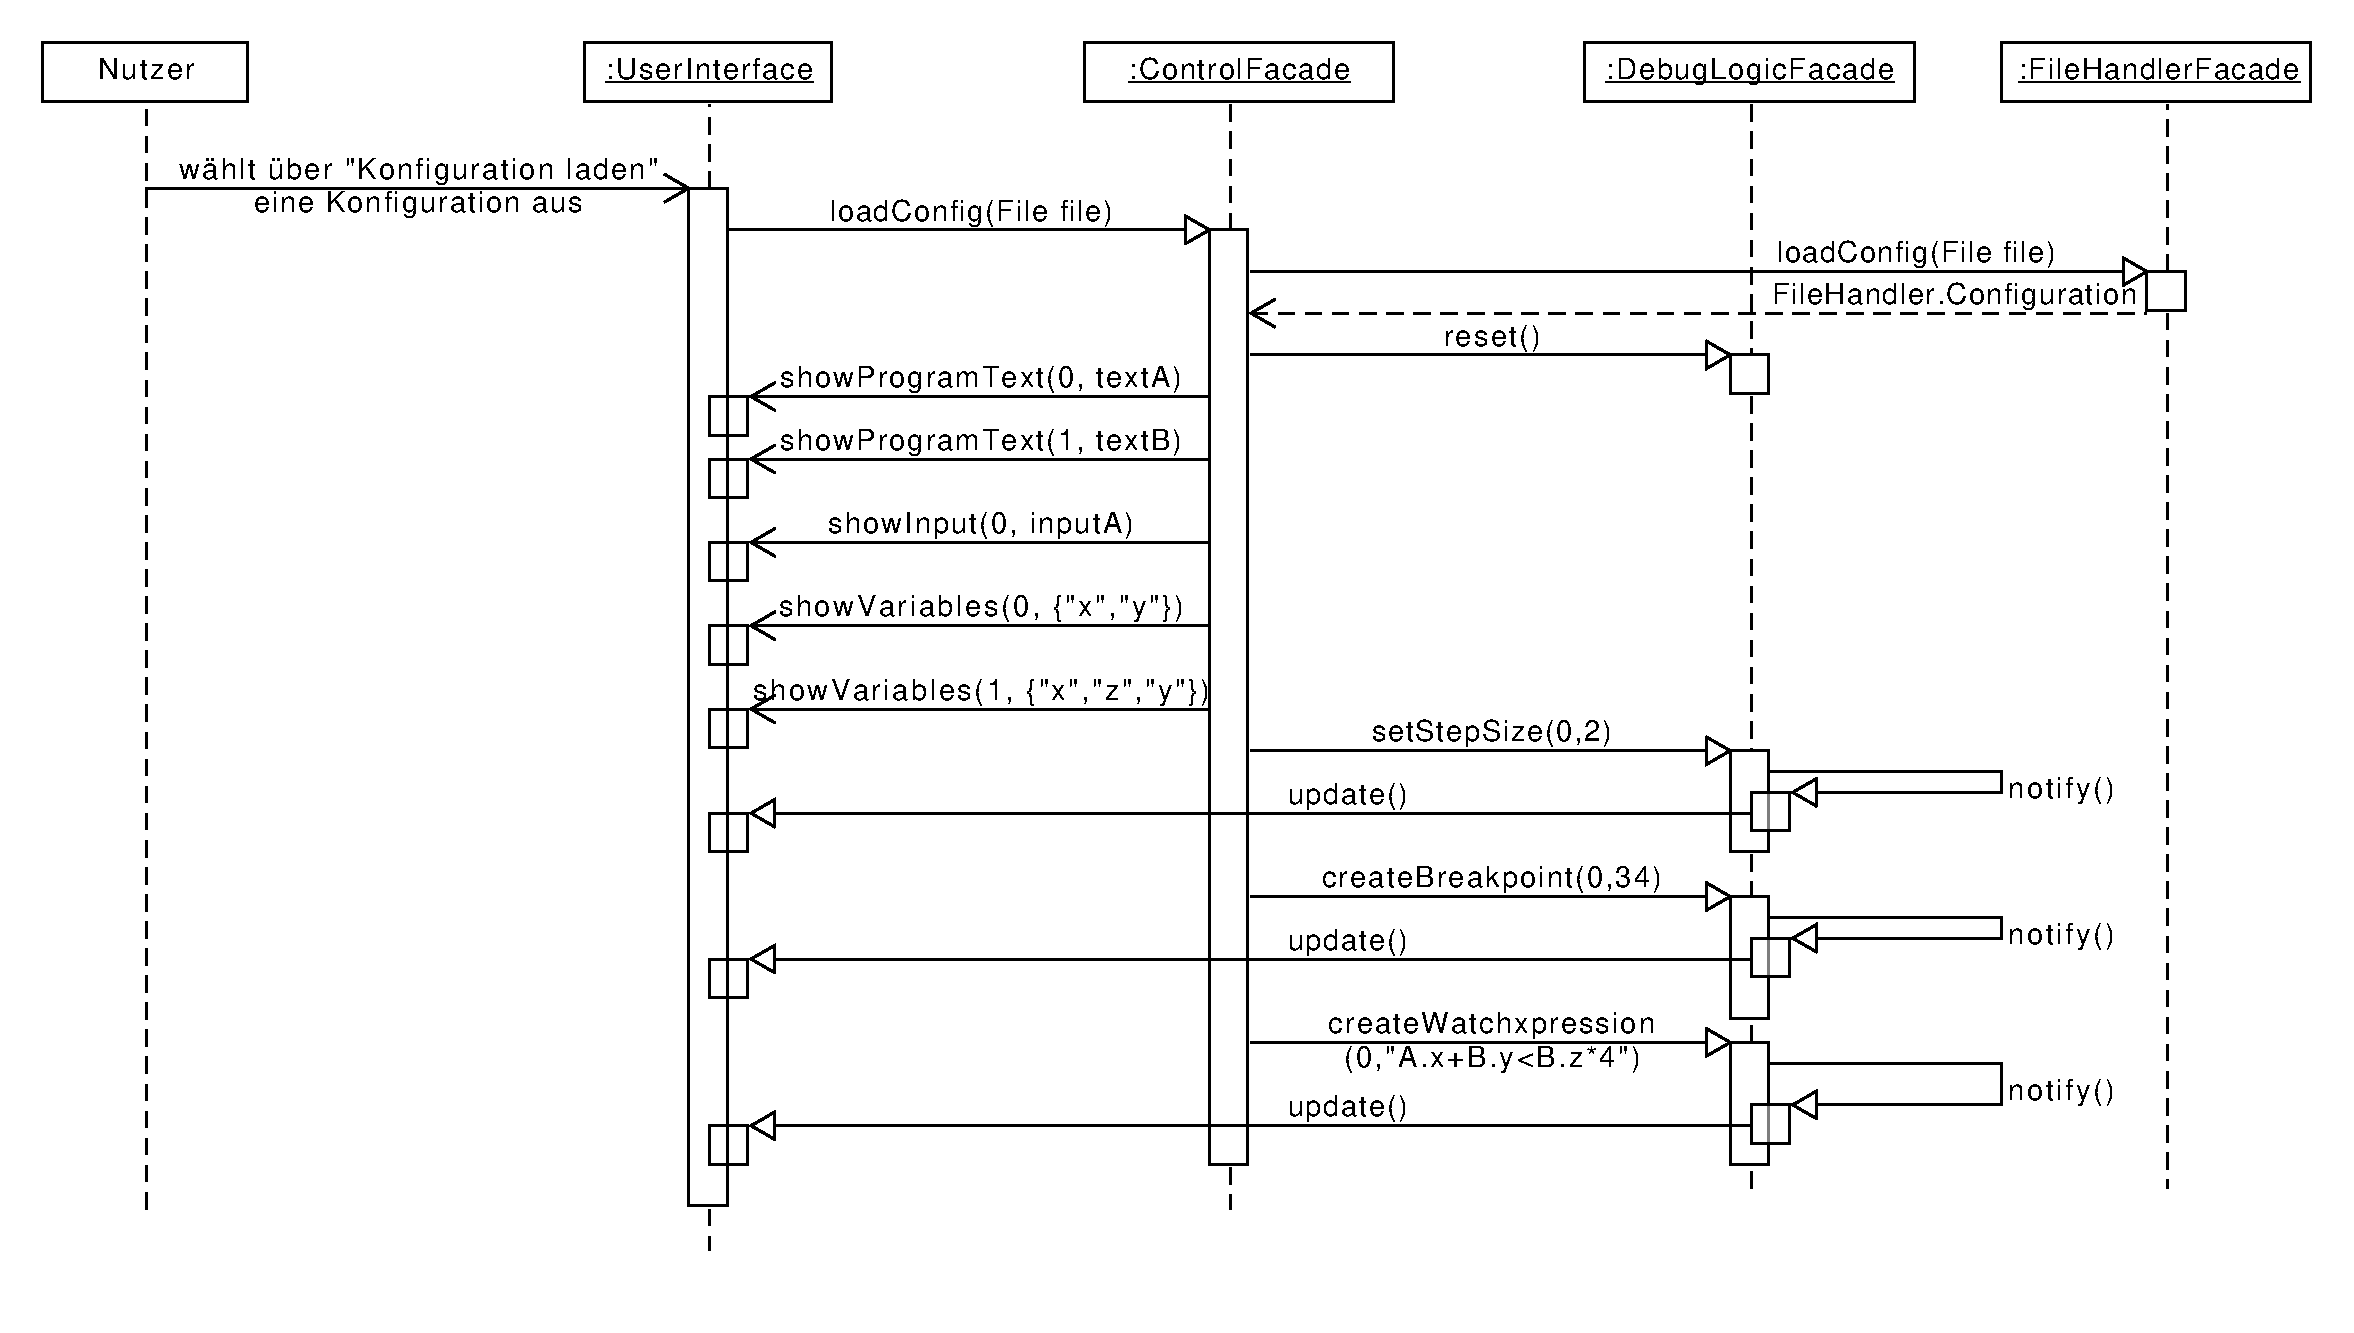
\includegraphics[width=0.8\textwidth]{diagrammIdeenUmlet/SequenceDiagrams/seq_loadConfigPDF.pdf}
\caption{Sequenzdiagramm:  Laden einer Konfigurationsdatei}
\end{figure}
Wählt der Benutzer über den Menpeintrag \enquote{Konfigurationsdatei laden} eine Konfiguration aus,
gibt das UserInterface diesen Befehl an die Control weiter, welche ein Configuration Objekt vom FileHandler 
erhält. \\
Die Control ruft anschließend Methoden der GUIFacade auf, um die Programmtexte, Eingabevariablen und
die im Variableninspektor anzuzeigende Variablen anzuzeigen. Außerdem ruft die Control
Mathoden der DebugLogicFacade auf, um für jedes Programm die Breakpoints, Watch-Expressions und
Schrittgrößen festzulegen. Über diese Änderungen wird das UserInterface als Observer benachrichtigt und
kann diese ebenfalls anzeigen

\newpage
\subsection{Konfigurationsdatei speichern}
\begin{figure}[!h]
\centering
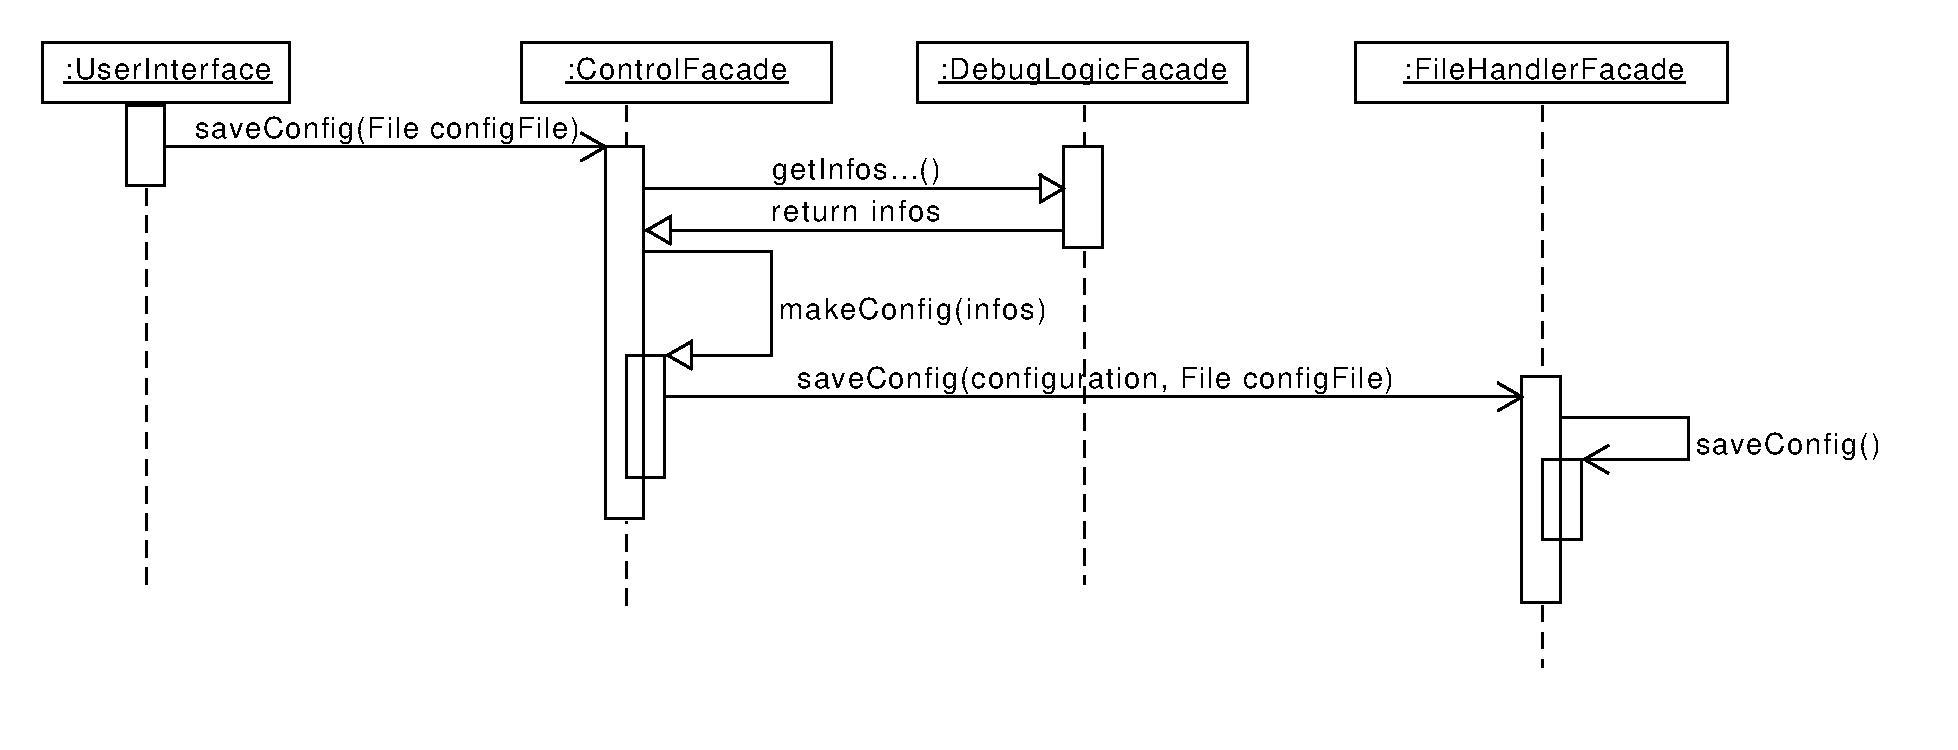
\includegraphics[width=0.8\textwidth]{diagrammIdeenUmlet/SequenceDiagrams/seq_saveConfigPDF.pdf}
\caption{Sequenzdigramm: Speichern einer Konfigurationsdatei}
\end{figure}
Möchte der Benutzer eine Konfigurationsdaatei speicher, reicht das UserInterface den Speicherort
an die ControlFacade weiter. Die Control sammelt die benötigten Daten in einer Configuration Instanz.
Dieses Objekt wird mit dem angegebenen Speicherort an die FileHandlerFacade weitergegeben, welche 
dann die Konfigurationsdatei auf dem Rechner des Benutzers speichert.

\newpage
\subsection{AF10: Hinzufügen von Programmen}
\begin{figure}[!h]
\centering
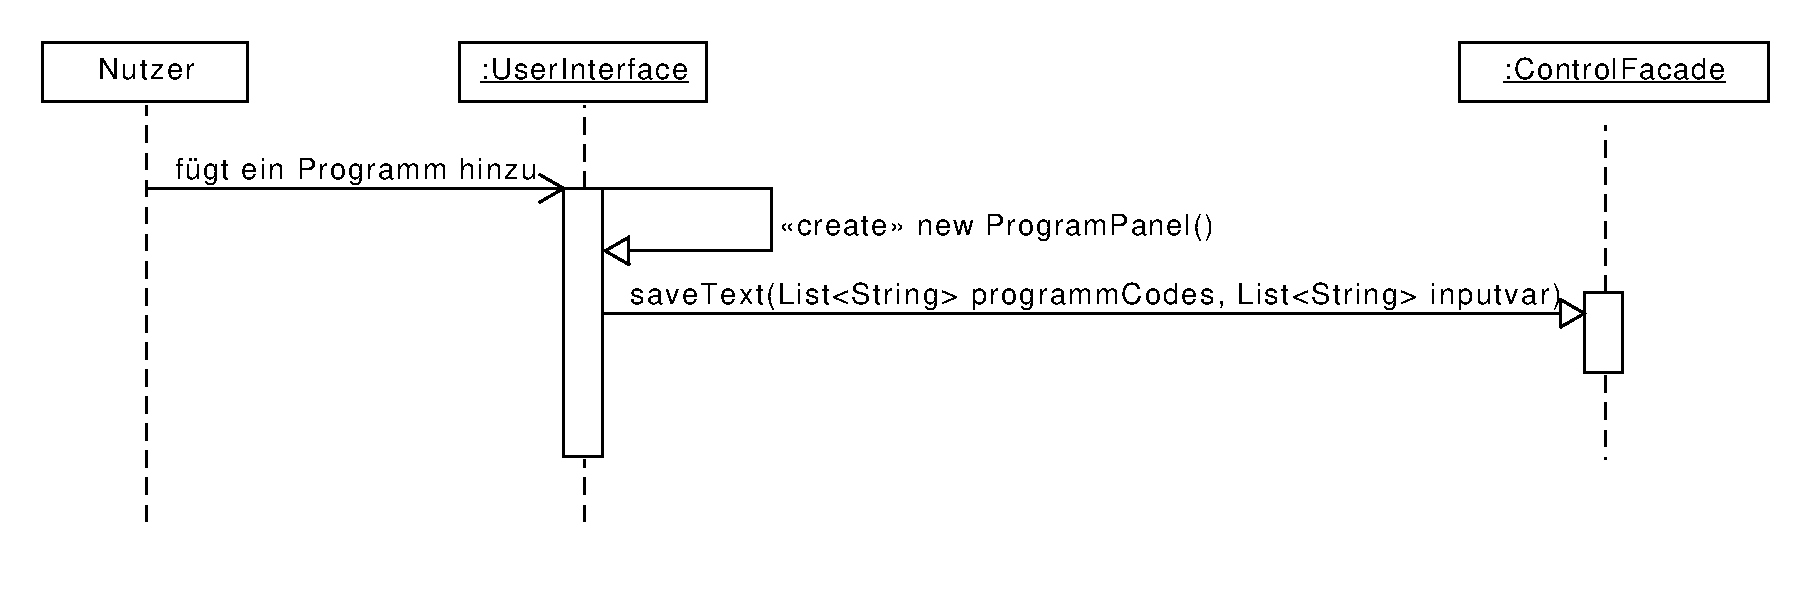
\includegraphics[width=0.8\textwidth]{diagrammIdeenUmlet/SequenceDiagrams/seq_AF10PDF.pdf}
\caption{Sequenzdiagramm: Hinzufügen von Programmen}
\end{figure}
AF10 ist falsch


\newpage
\subsection{AF20: Ändern von Programmen}
\begin{figure}[!h]
\centering
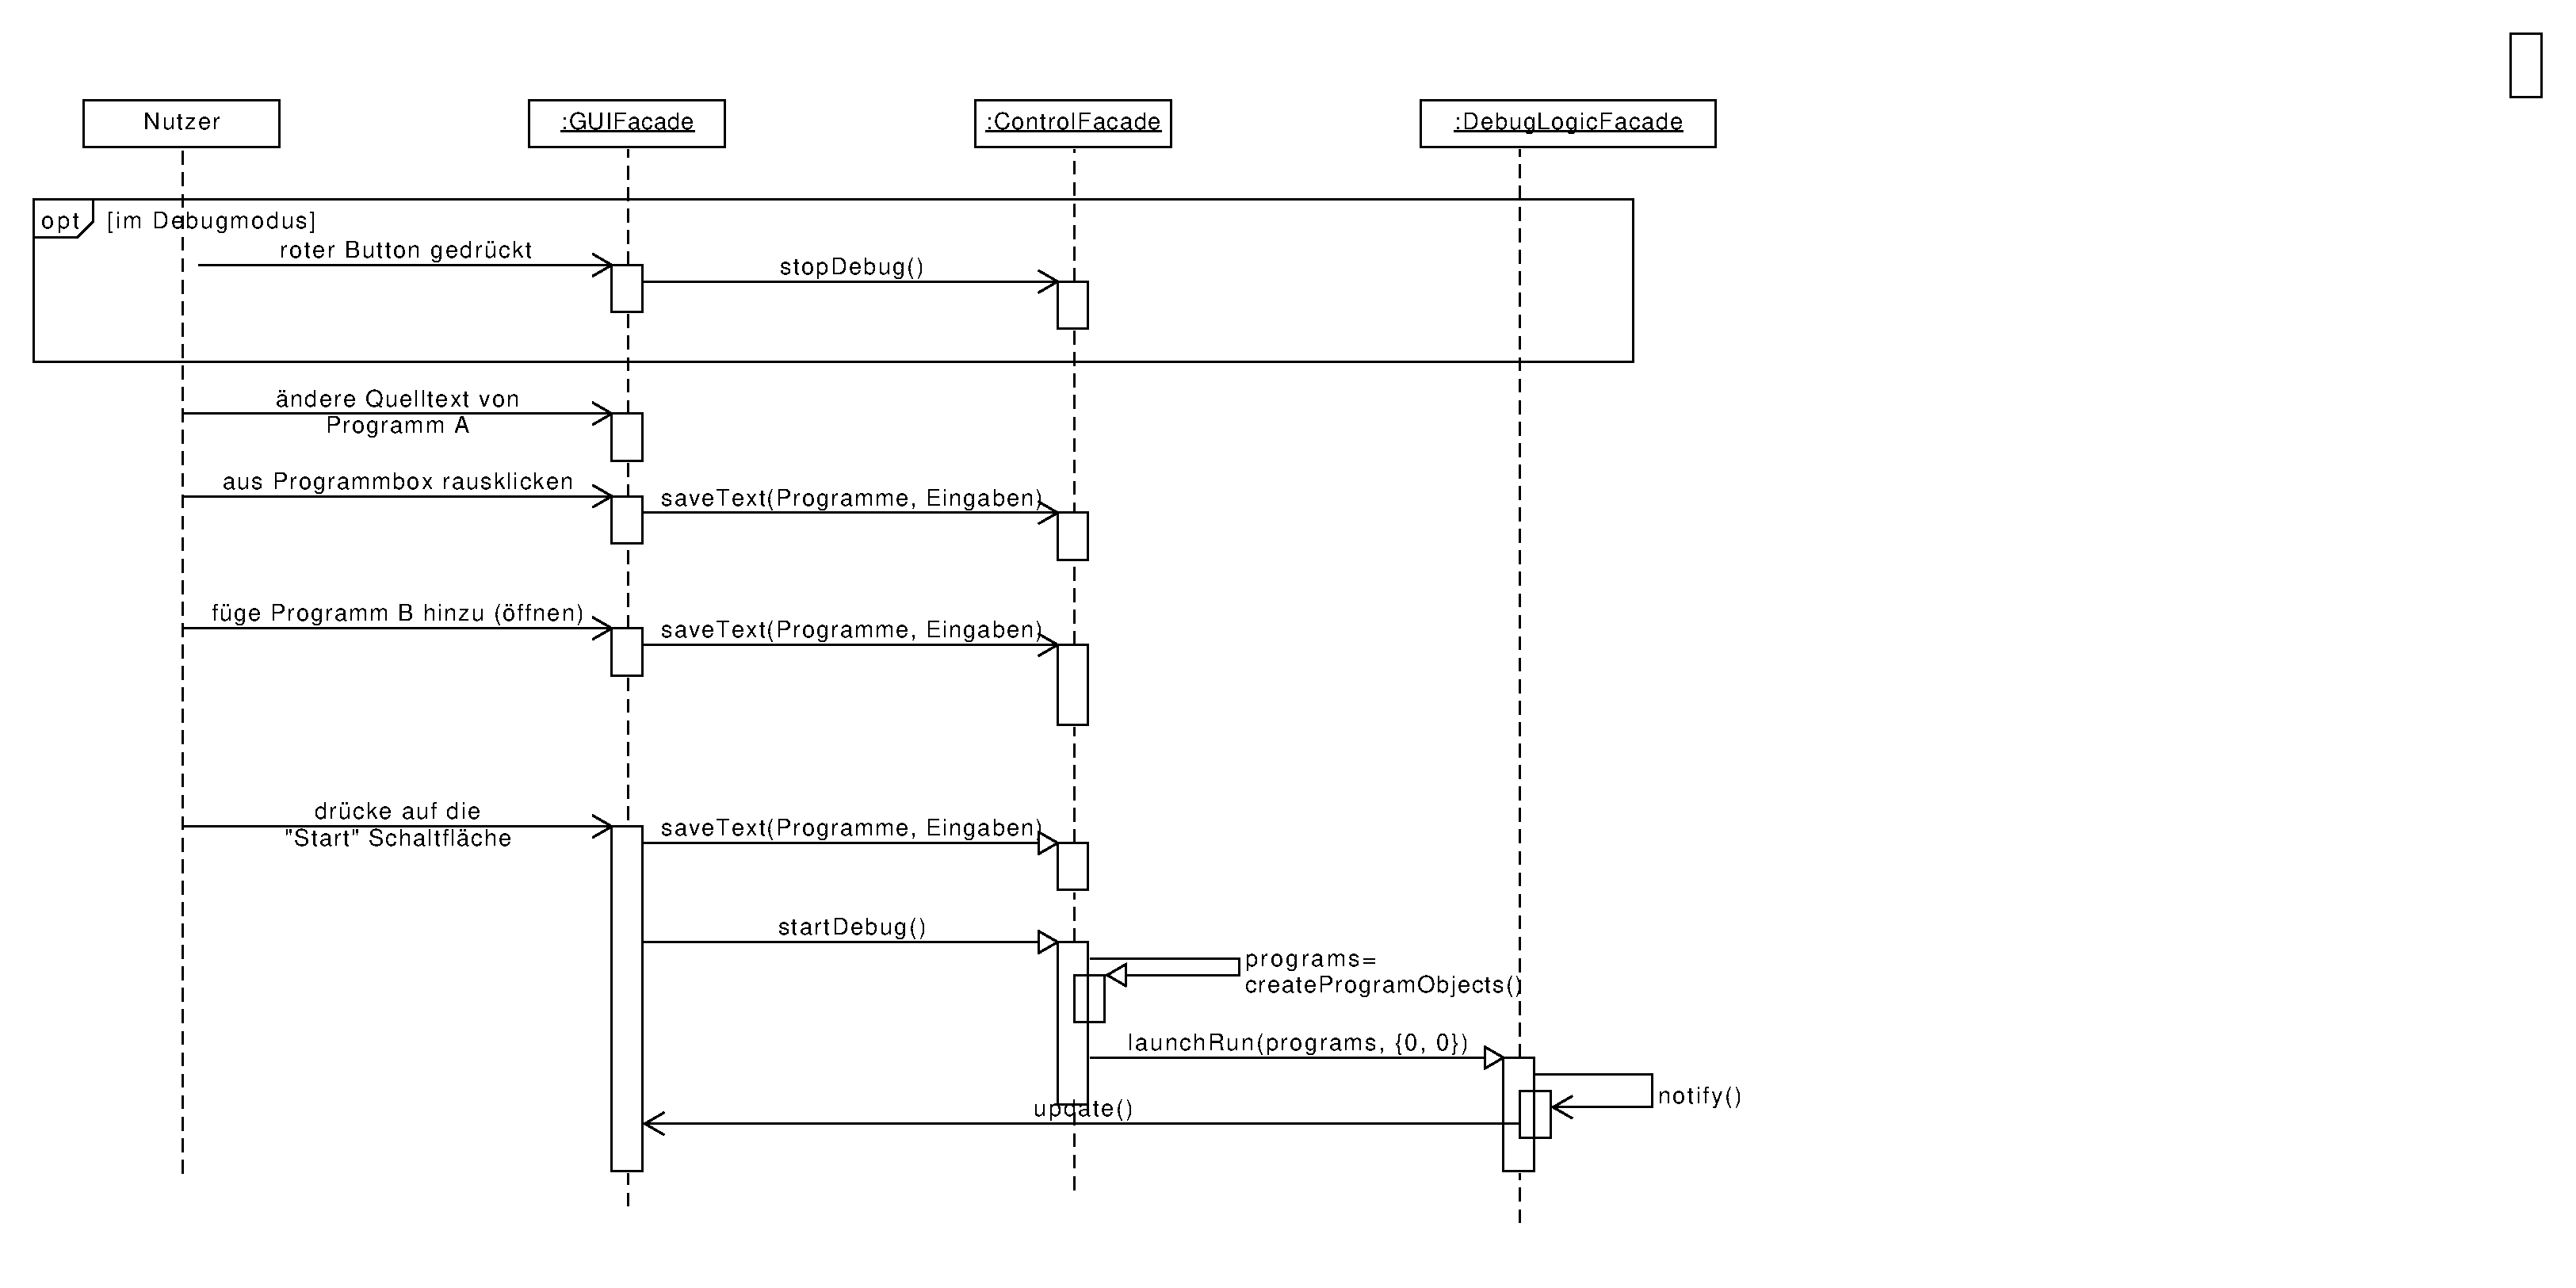
\includegraphics[width=0.8\textwidth]{diagrammIdeenUmlet/SequenceDiagrams/seq_AF20PDF.pdf}
\caption{Sequenzdiagramm: Ändern von Programmen}
\end{figure}
Möchte der Benutzer einen Programmtext editieren, muss er gegebenenfalls zunächst den Debugmodus beenden.
Anschließend lässt sich der Programmtext im Textfeld bearbeiten. Sobald der Benutzer außerhalb des
Textfelds klickt, gibt das MainInterface den neuen Programmtext und die Eingabeavariablen an die ControlFacade weiter. \\
Fügt der Benutzer einen neuen Programmtext durch Öffnen einer Datei hinzu, gibt das MainInterface diesen ebenfalls
mit den angegebenen Eingabevariablen an die ControlFacade weiter.\\
Sobald der Benutzer die Start-Schaltfläche auswählt um den Debugmodus zu starten, gibt das MainInterface erneut
alle eingegebenen Texte weiter und ruft schließlich startDebug() der ControlFacade auf. Diese erstellt aus den gespeicherten Informationen
Programm-Instanzen und gibt diese an die DebugLogicFacade weiter und startet damit den Debug-Lauf.

\newpage
\subsection{AF30: Setzen von Breakpoints}
\begin{figure}[!h]
\centering
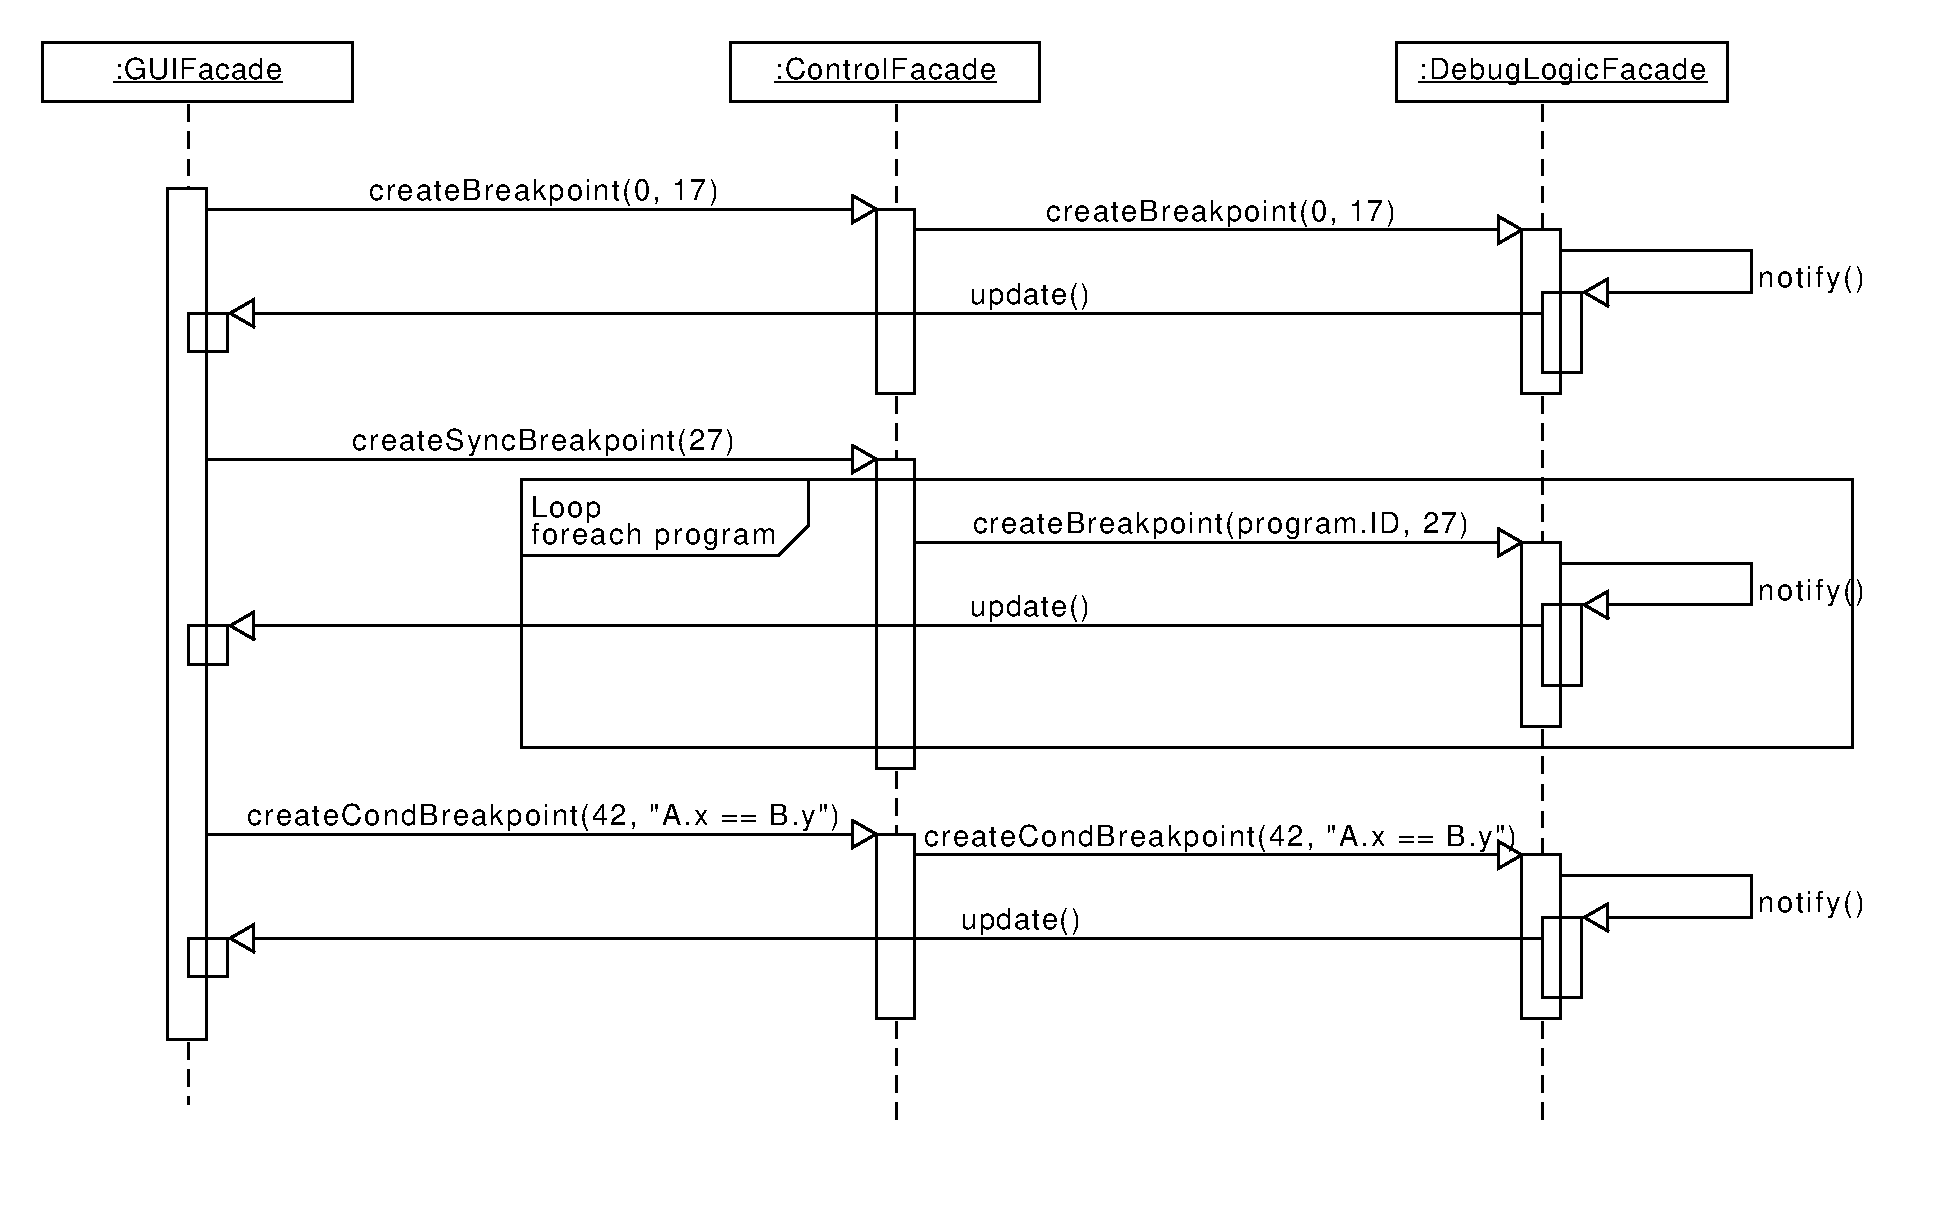
\includegraphics[width=0.8\textwidth]{diagrammIdeenUmlet/SequenceDiagrams/seq_breakpointsPDF.pdf}
\caption{Sequenzdiagramm: Setzen von Breakpoints}
\end{figure}
Setzt der Benutzer einen Breakpoint in eine Zeile in einem Programm, reicht das MainInterface
diese Information an die ControlFacade weiter, welche dann createBreakpoint mit der Programm-ID und der
Zeile an die DebugLogicFacade weitergibt.
Setzte der Benutzer jedoch einen Breakpoint in allen Programmen, teilt das
MainInterface dies der ControlFacade mit. Die ControlFacade ruft für jedes Programm
die Methode createBreakpoint der DebugLogicFacade auf.
Beim hinzufügen von bedingten Breakpoints gibt das MainInterface die ID des Breakpoints
und den vom Benutzer angegebenen Ausdruck an die ControlFacade weiter. Die Control reicht diese Informationen
ihrerseits an die DebugLogicFacade weiter, welche den Breakpoint ab diesem Zeitpunkt auswertet.

\newpage
\subsection{AF40: Hinzufügen von Watch-Expressions}
\begin{figure}[!h]
\centering
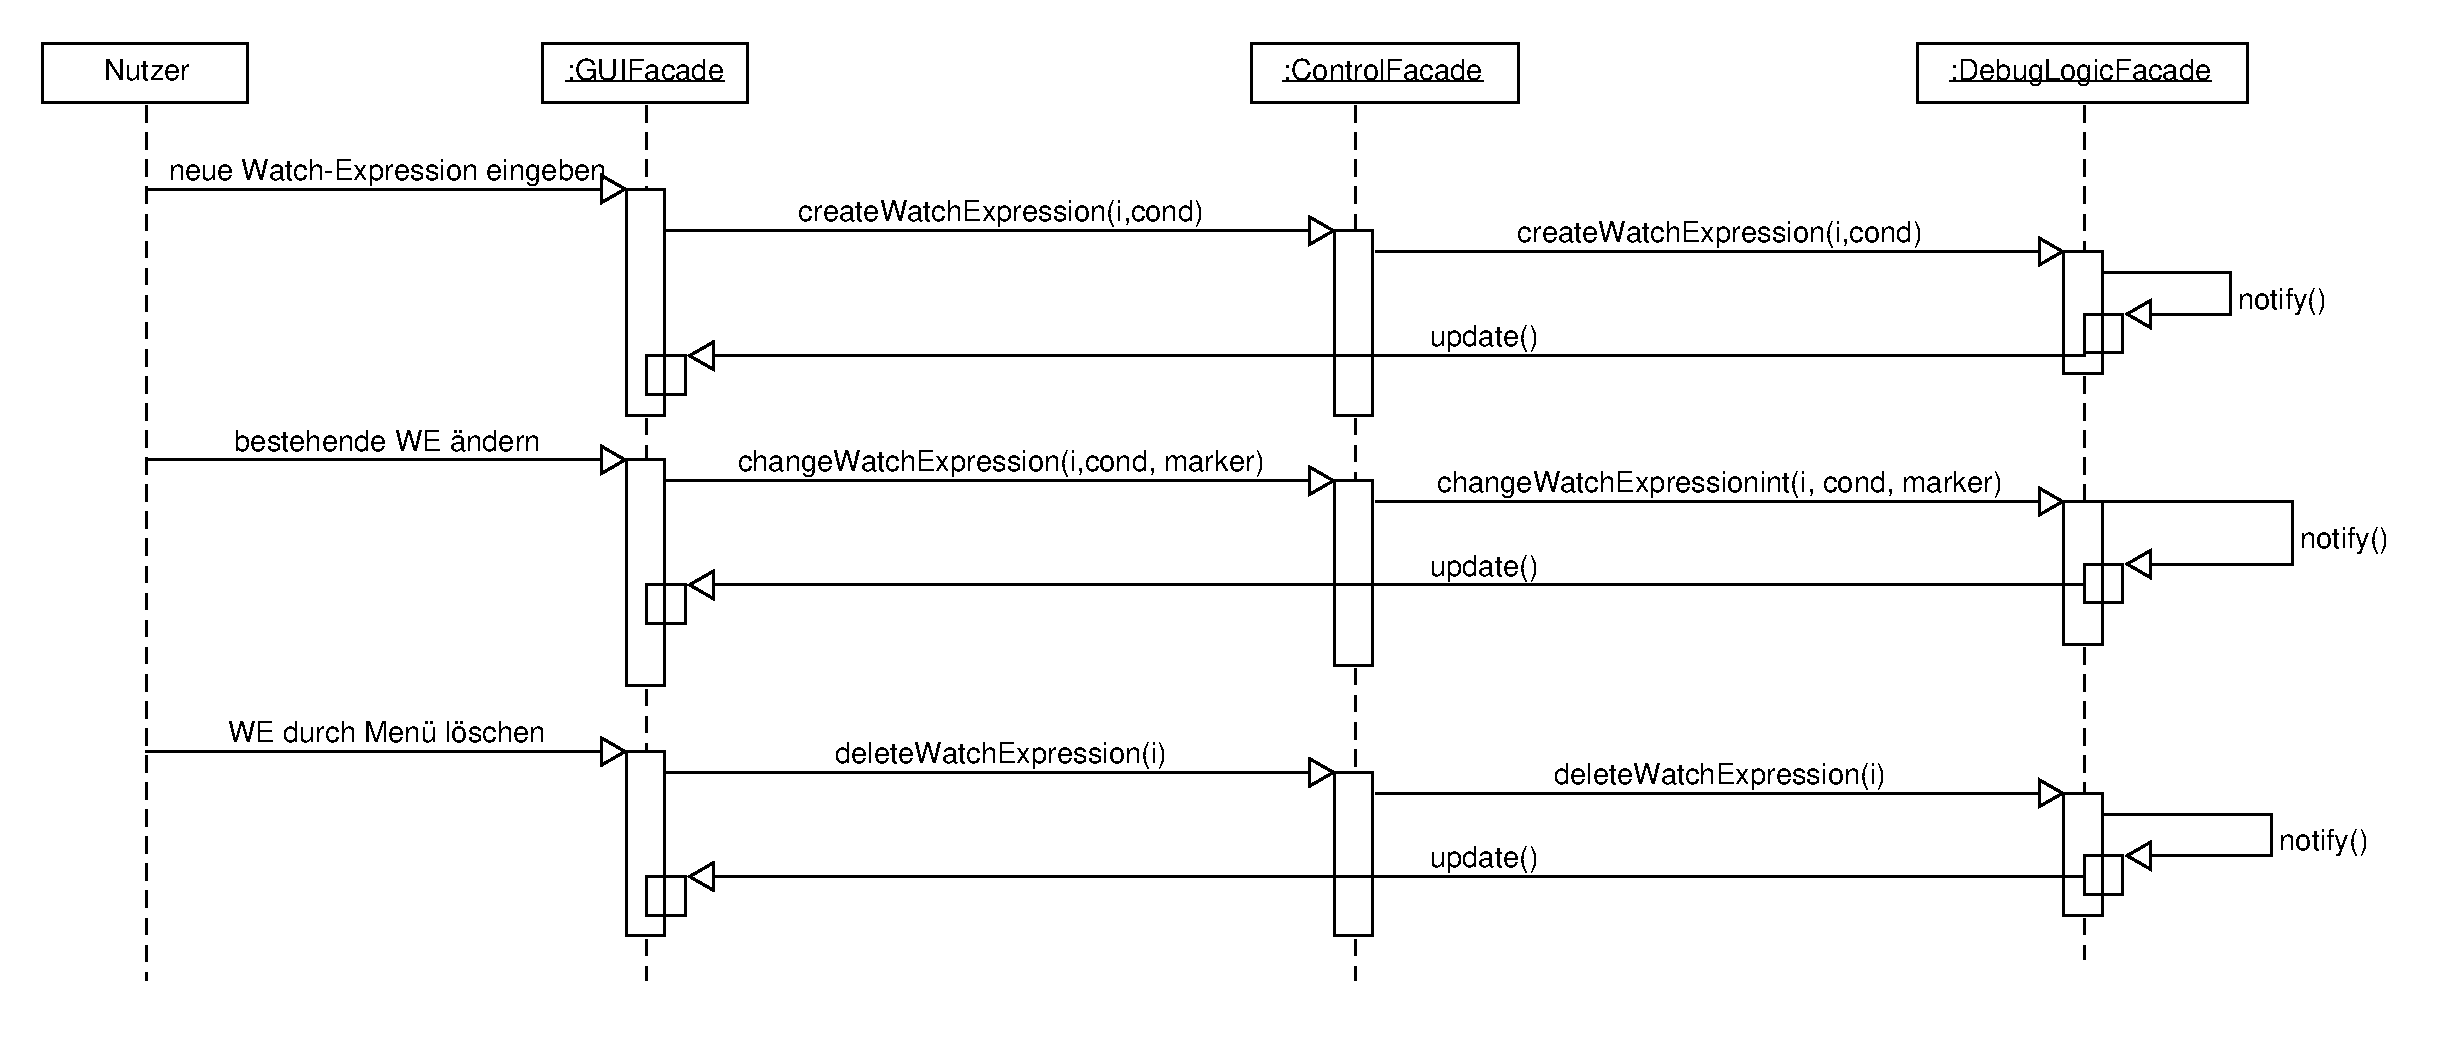
\includegraphics[width=0.8\textwidth]{diagrammIdeenUmlet/SequenceDiagrams/seq_WatchExpressionsPDF.pdf}
\caption{Sequenzdiagramm: Hinzufügen von Watch-Expressions}
\end{figure}
Dieser Vorgänge sind für Watch-Expressions und bedingte Breakpoints identisch. \\
Gibt der Benutzer eine neue Watch-Expression an, wird die Bedingung und die ID vom MainInterface über 
die Control an die DebugLogicFacade weitergegeben. Ändert der Benutzer die Watch-Expression, zB indem 
er die Bereichsbindung angibt, wird dies ebenfalls über die Control an die DebugLogicFacade weitergegeben.
Auch beim Löschen einer Watch-Expression über das entsprechende Menü der Benutzeroberfläche, erhält die
DebugLogic diese Information über die Control und stoppt das Auswerten dieser Watch-Expression.

\newpage
\subsection{AF50: Programme debuggen}
\begin{figure}[!h]
\centering
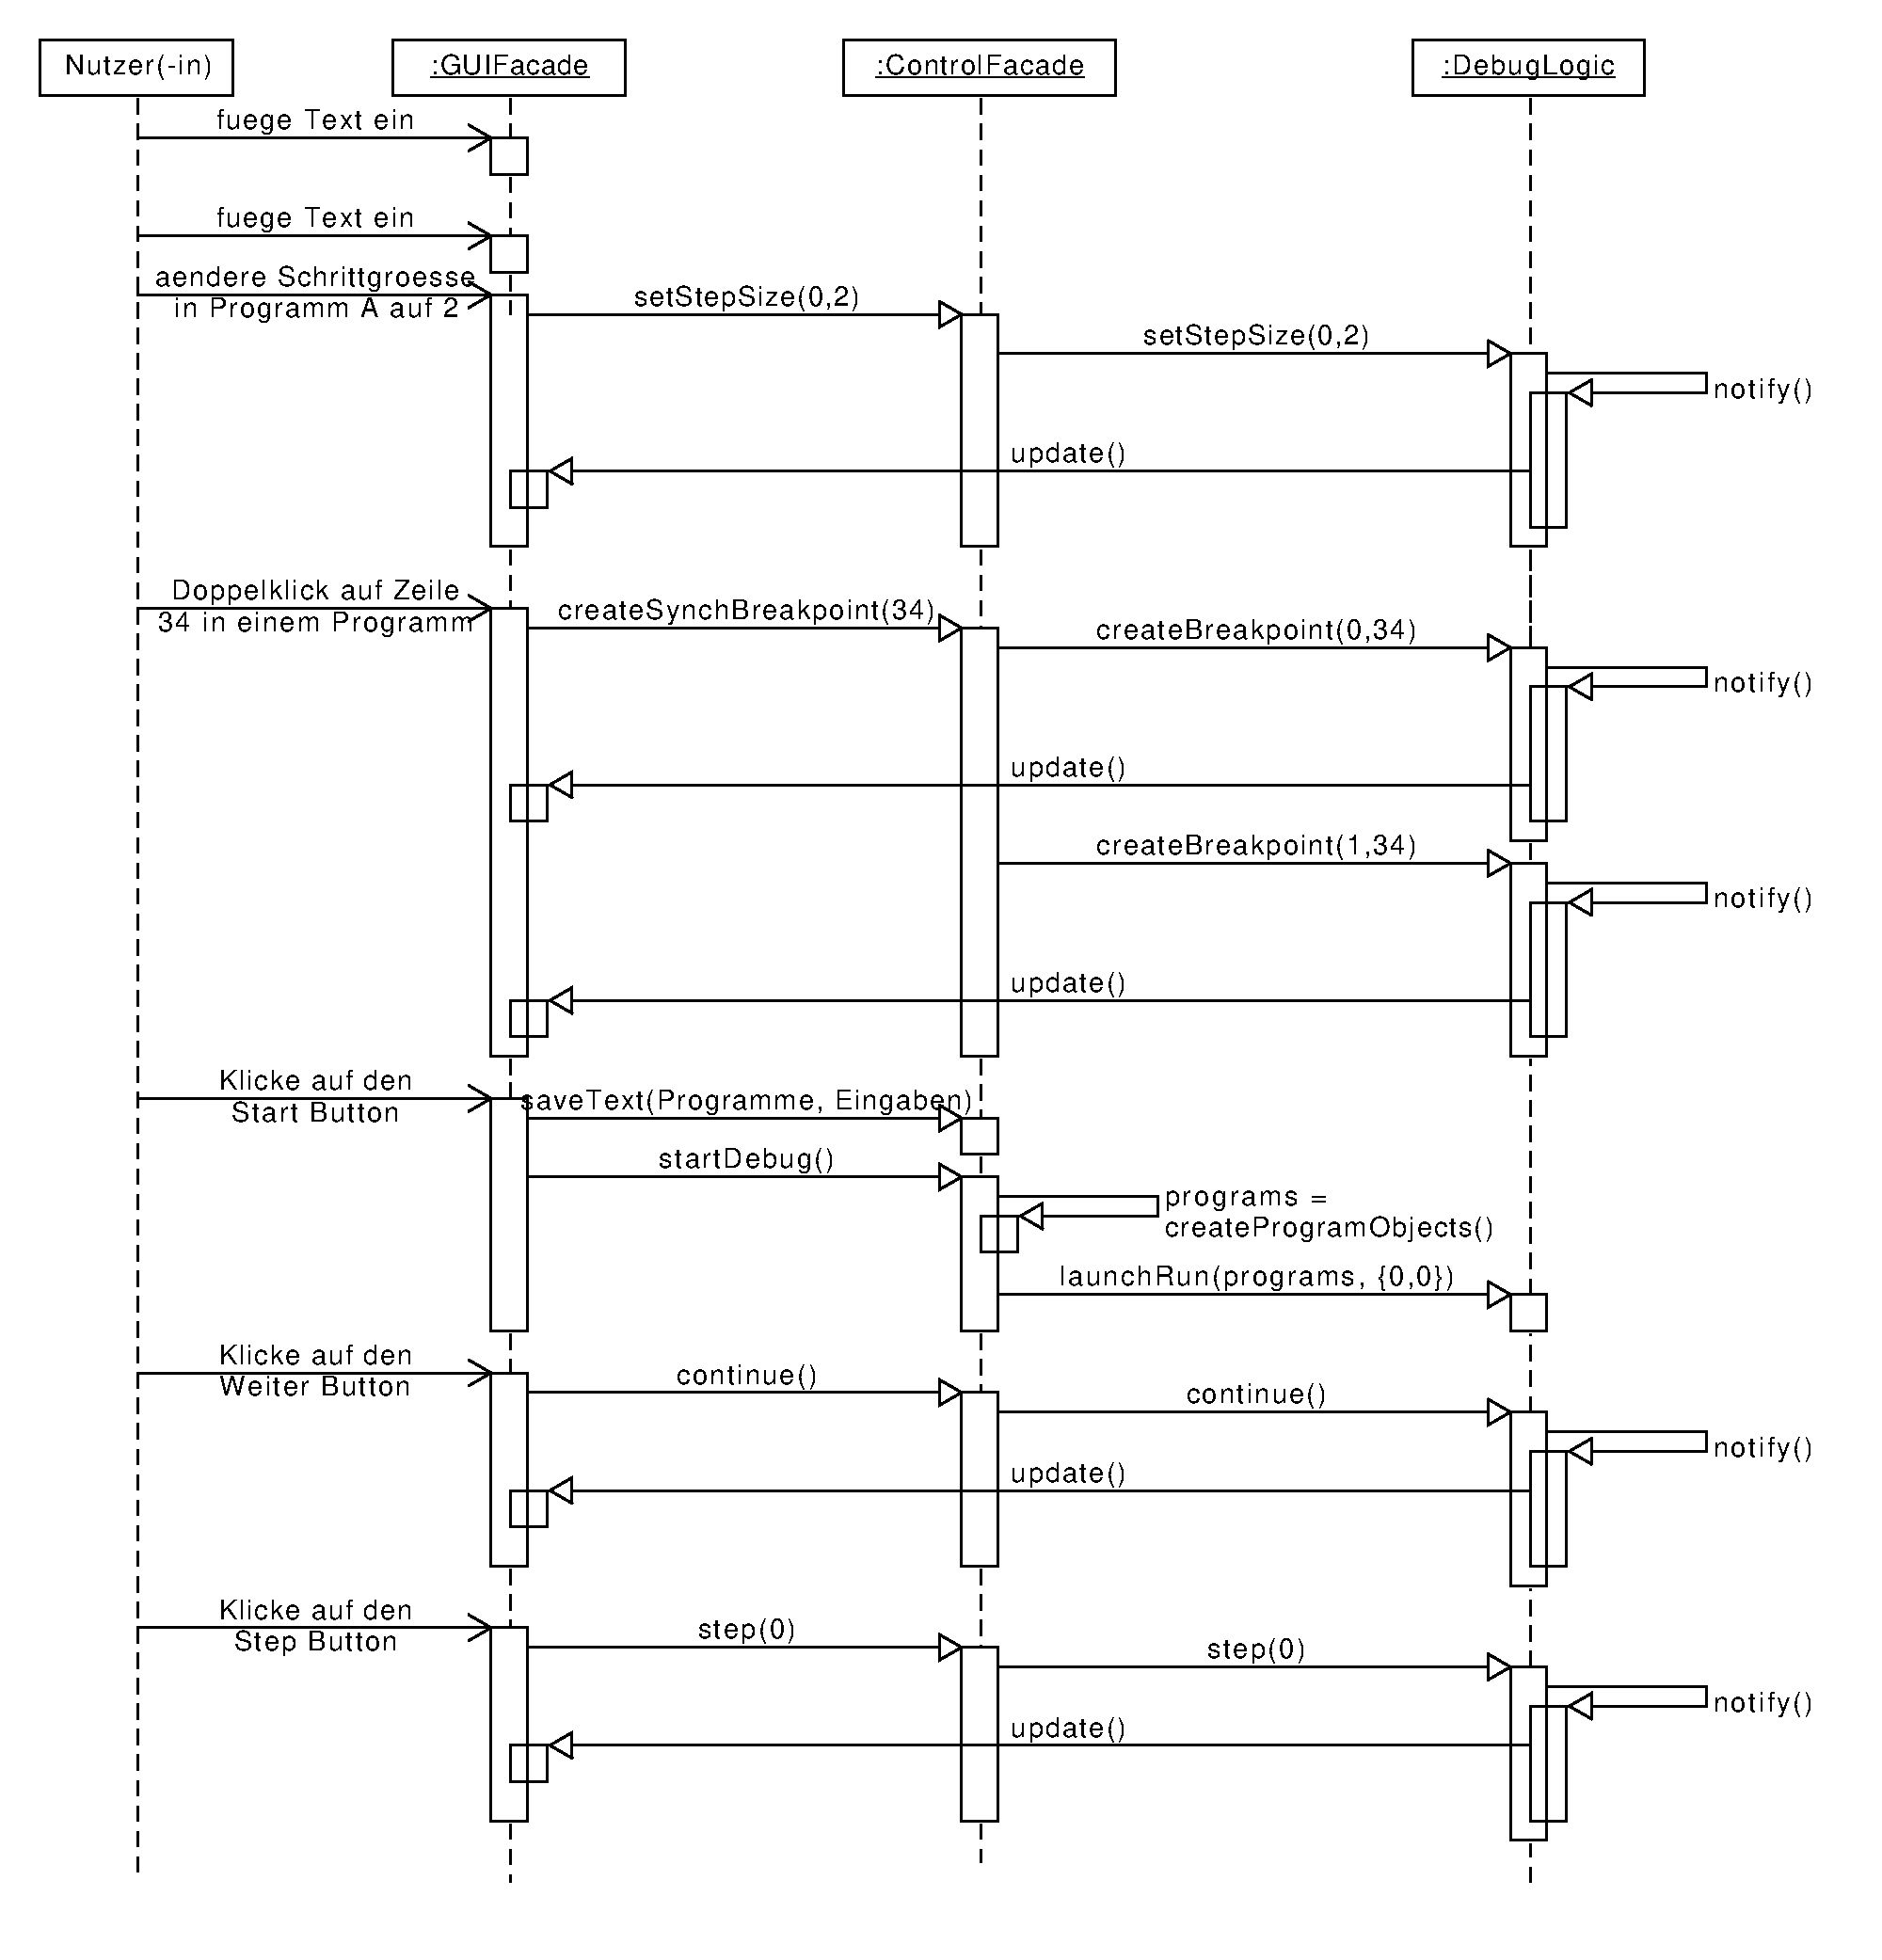
\includegraphics[width=0.8\textwidth]{diagrammIdeenUmlet/SequenceDiagrams/seq_AF50PDF.pdf}
\caption{Sequenzdiagramm: Debuggen von Programmen}
\end{figure}
Dieses Sequenzdiagramm fasst die Schritte des Nutzers bei einem Debug-Lauf zusammen.
Hierbei werden zuvor Programme hinzugefügt, die Schrittgröße geändert und Breakpoints hinzugefügt.
Sobald der Benutzer auf Start klickt, werden seine Eingaben final gespeichert und die Control startet 
den DebugLauf der DebugLogic.
Wenn der Benutzer durch Weiter oder Schritt durch den DebugLauf navigiert, werden diese Befehle über
die Control an die DebugLogic weitergegeben. Die Schritte werden von der DebugLogic ausgeführt, und anschließend
wird die GUIFacade als Beobachter dazu aufgefordert, die aktualisierten Werte anzuzeigen.

\newpage

\section{Abhängigkeitseinteilung mit Blick auf die Implementierung}
%Mit Blick auf den Implementierungsplan: Aufteilung in Klassen/Pakete, die unabhängig voneinander implementiert und getestet werden können.
\subsection{Abhängikeiten}
Das Paketdiagramm besagt, dass FileHandler und DebugLogic nicht voneinader abhängen.
Beide werden von der Control benutzt und müssen somit korrekt implementiert sein, bevor die Control richtig funktionieren kann. Weiter führt die Control Methoden der GUIFacade aus, ist aber nicht von derer Abhängig, da diese nicht relevant ist für eine funktionierende Control.
Die GUI hingegen ist stark von der Control abhängig und kann ohne diese nicht korrekte Daten anzeigen.

%TODO Pakete der Debuglogic aktualisieren, da noch nicht fertig
\subsection{Implementierung}
Die Implementierung der Hauptpakete kann durch den von Fassaden geprägten Entwurf und dem MVC-Konzept gleichzeitig geschehen. Es ist jedoch sinnvoll das Exception Paket als erstes zu implementieren, um später keine Stellen im Quelltext suchen zu müssen, an denen Fehler auftreten können.
Weiter sollten die Unterpakete der DebugLogic entsprechend der Benutztrelation implementiert werden, also zuerst AntlrParser, Interpreter und zum Schluss der Debugger.
Dieses Problem besteht bei den Hauptpaketen nicht, da für die Kommunikation ausschließlich Fassaden benutzt werden. Diese können zur gleichzeitigen Implementierung der Pakete als Stummel pseudoerstellt werden, d.h. die Methoden sind leer und enthalten keine bzw. nur sehr wenig Funktionalität.\\
Der FileHandler stellt wiederum eine Ausnahme dar, da er mehrere Klassen zur Repräsentation und Interaktion zum Dateisystem bereitstellt.
Hierbei müssen die Klassen ConfigurationFile, PropertiesFile und LanguageFile gleichzeitig mit der FileHandlerFacade Klasse einsatzbereit sein.

\begin{figure}[!h]
\centering
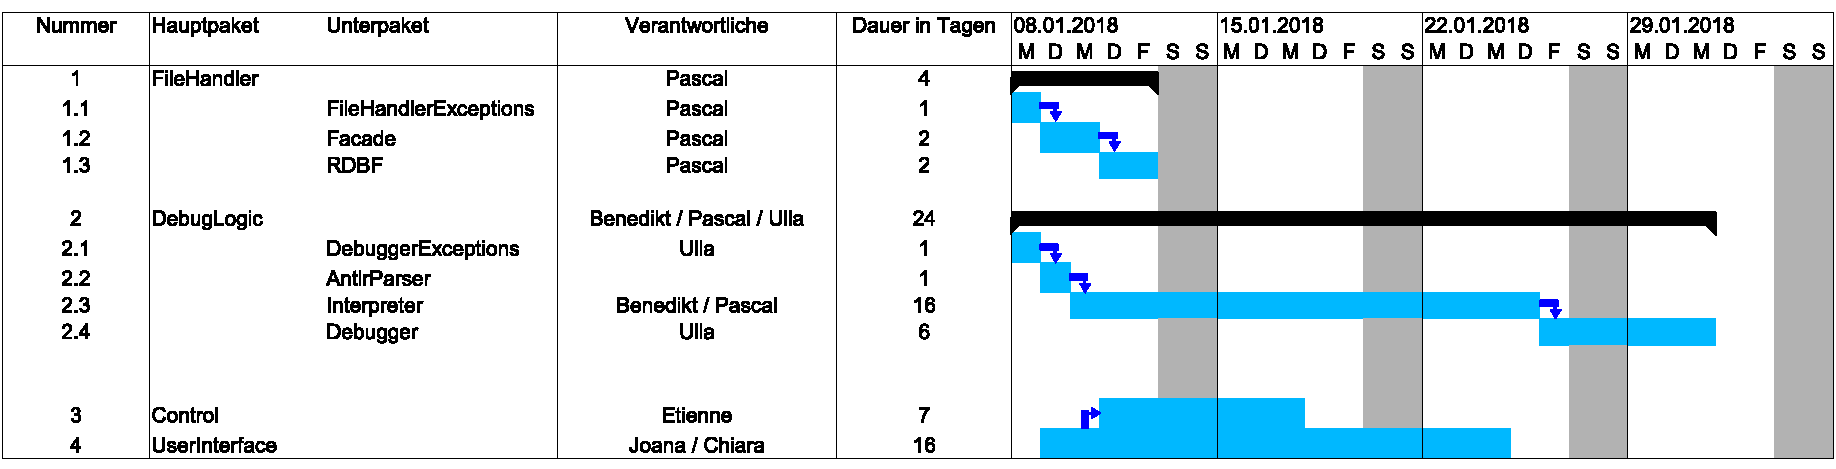
\includegraphics[width=1.0\textwidth]{GanttDiagramm_withArrows.pdf}
\caption{Gantt Diagramm: Zeitplanung der Implementierung}
\end{figure}


\section{Formale Spezifikation von WLang und Speicherformaten}\label{FormSpez}
Speicherformate, Sprachdefinition(formal)

\section{Änderung zum Pflichtenheft}
Änderungen zum Pflichtenheft, z.B. gekürzte Wunschkriterien.




\section{Anhang}
UML-Klassendiagramm 
Vollständiges großformatiges Klassendiagramm im Anhang. Ausschnitte/Teile können bereits
vorher verwendet werden, um Teilkomponenten zu beschreiben. Assoziationen zwischen Klas-
sen dabei bitte mit entsprechenden Pfeilen darstellen, statt nur durch Feldtypen.






\end{document}
\grid
\grid
